\documentclass[11pt]{article}
\usepackage{icmlko}
\begin{document}

\title{축을 세면 비선형이 보인다 --- 라벨 없이 읽히는 대리물 하나, 그리고 끊긴 사슬}
\author{월드모델 실험실}
\date{노트 411 · 2026년 8월 2일}
\maketitle

\begin{abstract}
노트 410이 용량 축의 정체를 \textbf{비선형 요구}로 밝히면서 벽을 하나 남겼다
--- 그 값을 재려면 \textbf{그 도메인의 라벨이 있어야 한다}(선형과 비선형을
둘 다 적합해서 뺀다). 안 본 도메인에는 라벨이 없다. \textbf{라벨 없이 읽을
수 있는 대리물}이 있으면 전이 쪽 벽이 하나 뚫린다.

대리물을 \textbf{하나만} 사전 등록했다 --- \emph{그 도메인에서 실제로
관측되는 축의 개수}. 축이 많을수록 상호작용이 있을 자리가 많다. 여럿을
훑고 제일 잘 맞는 것을 고르면 노트 401의 $-0.564$ 가 다시 나온다.

\begin{center}
\begin{tabular}{lrr}
\hline
 & 관측 축 수 & 비선형 요구 \\
\hline
웹툰 & $16$ & $+0.1050$ \\
모바일 & $13$ & $+0.1637$ \\
펀딩 · 아이돌 & $12$ & $+0.2685$ · $+0.2204$ \\
$\cdots$ & & \\
팝업 & $5$ & $\mathbf{-0.0478}$ \\
만화 & $4$ & $+0.0122$ \\
시장팝업 & $3$ & $\mathbf{-0.0189}$ \\
\hline
\end{tabular}
\end{center}

$\rho = \mathbf{+0.781}$ --- 사전 등록 문턱 $|0.5|$ 를 넘었다. 두 양은
\textbf{공유항이 없다}(하나는 자료의 성질, 하나는 두 모형의 차). 비선형이
음수인 유이한 도메인이 축 셋·다섯짜리다.
\end{abstract}

\section{그런데 사슬이 안 이어진다}

정직하게 적어야 할 것이 있다. 사슬의 두 마디는 각각 튼튼하다 ---
\textbf{축 수 $\to$ 비선형} $+0.781$, \textbf{비선형 $\to$ 용량 선호}
$+0.773$(노트 410). 그런데 \textbf{축 수 $\to$ 용량 선호}를 곧바로 재면
$\mathbf{+0.297}$ 이다.

끊는 것은 \textbf{웹툰}이다. 축이 열여섯으로 제일 많고 비선형도 넷째인데
용량 선호는 $+0.0020$ 으로 열째다. 노트 409에서 세 기계 모두에서 축의 반대
끝에 혼자 있었고, 노트 410의 시간 어긋남 가설도 그것을 못 설명했다
(연도 간격 $\leftrightarrow$ 잔차 $\rho = +0.037$). \textbf{같은 한 점이
세 번째로 걸린다.}

그래서 이 노트가 사는 것은 \textbf{반 칸}이다. 안 본 도메인에서 ``비선형이
얼마나 있을까''는 축을 세어 짐작할 수 있다. 그런데 ``그래서 깊이를 얼마나
줄까''는 아직 못 간다.

\section{사전 등록 안 한 것도 적는다}

같이 잰 두 가지: 한 번이라도 관측되는 축 수 $\rho = +0.706$, 관측 밀도
$\rho = \mathbf{+0.827}$. 밀도가 제일 높지만 \textbf{사전 등록한 것은 축
수다.} 셋 중 제일 좋은 것을 골라 적으면 그건 세 번 뽑아 이긴 것이지
$n{=}11$ 에서 잰 것이 아니다. 밀도는 \textbf{다음 사이클의 사전 등록
후보}로 남긴다.

\section{남은 것}

\begin{tabular}{lp{7.2cm}}
\hline
웹툰 (세 번째) & 축 수·비선형·시간 어느 것도 이 하나를 설명 못 한다.
판 무게 21\% 라 깊이 8 도 막고 있다 \\
관측 밀도 & $+0.827$ 이지만 사후에 본 것. 다음에 사전 등록해서 잰다 \\
선형이 나은 둘 & 팝업 · 시장팝업은 F18 이 F6 보다 낮다. 축이 셋·다섯뿐인
도메인엔 나무를 씌우지 말아야 할지 \\
\hline
\end{tabular}

\begin{figure}[h]
\centering
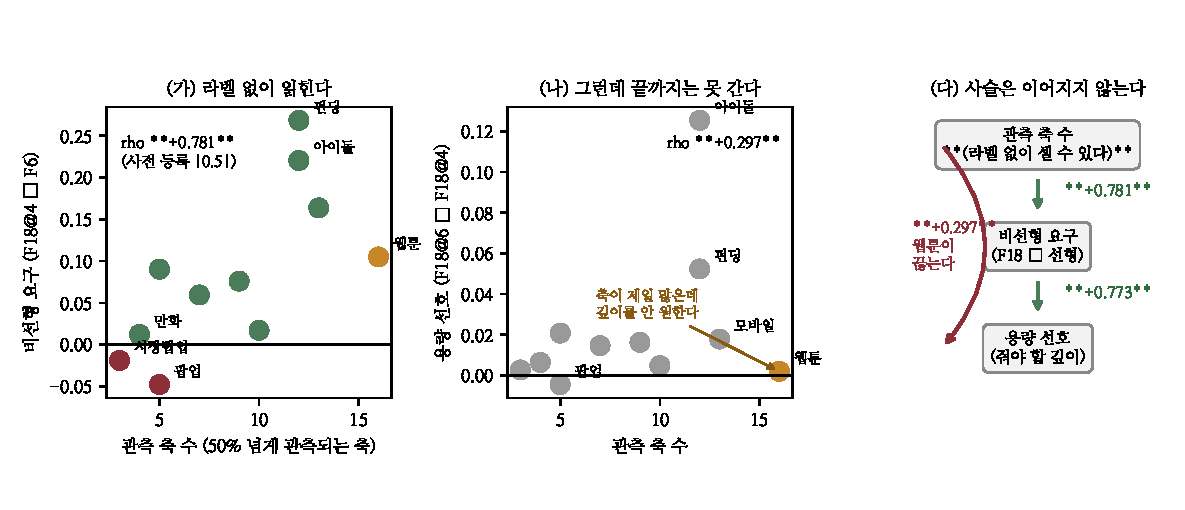
\includegraphics[width=\textwidth]{figs/fig411.pdf}
\caption{(가) 관측 축 수와 비선형 요구 ($\rho = +0.781$, 공유항 없음).
(나) 같은 축 수로 용량 선호를 재면 $+0.297$ --- 웹툰이 끊는다.
(다) 사슬: 두 마디는 튼튼한데 끝까지는 안 간다.}
\end{figure}

\end{document}
